% Chapter 1

\chapter{Future upgrades} % Main chapter title

\label{Chapter7} % For referencing the chapter elsewhere, use \ref{Chapter1} 
\section{Two AOM}
\begin{figure}
\begin{center}
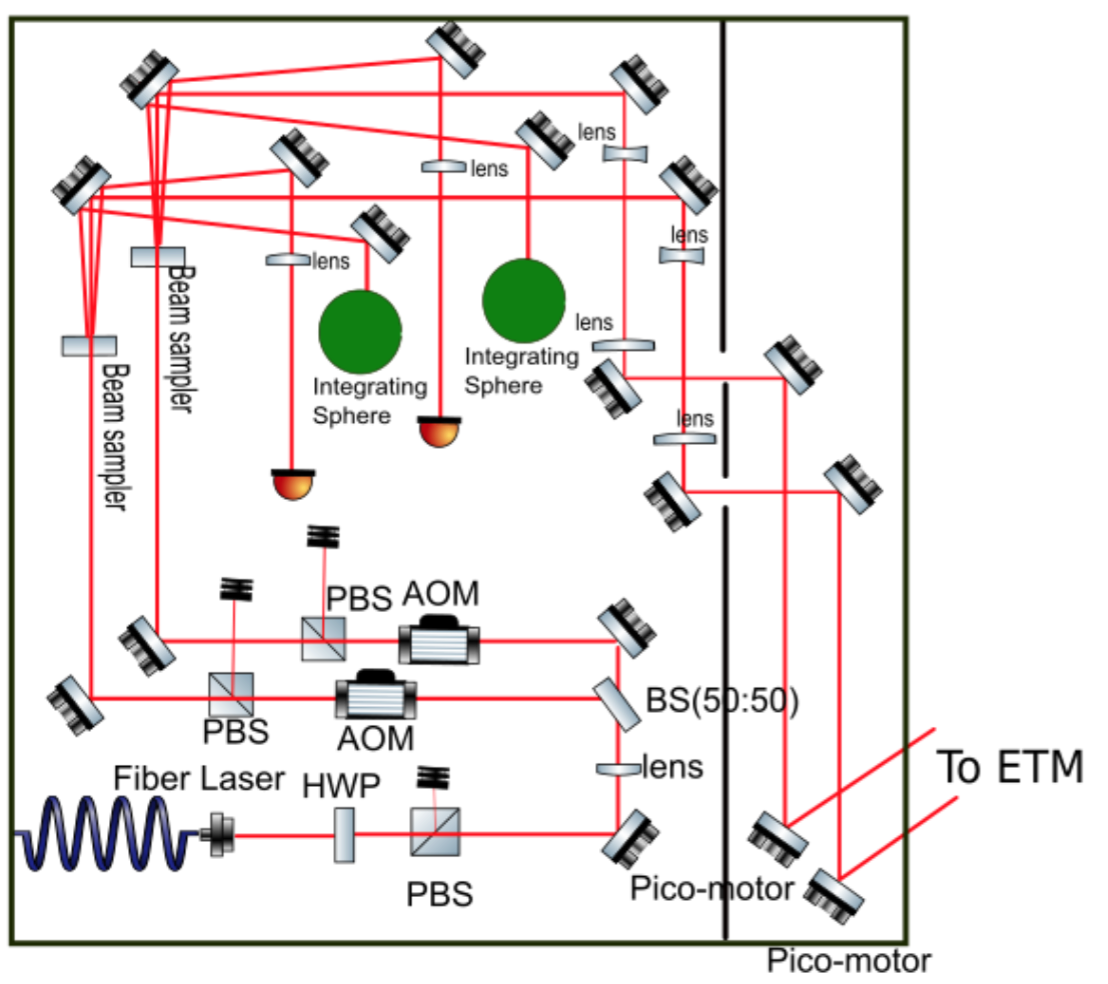
\includegraphics[width=14cm]{Figures/Adv_Tx_module_layout.eps}
\caption{.} 
\label{fig:Adv_Tx_module_layout} 
\end{center}
\end{figure}

\section{KAGRA Gold Standard}
Photo-detectors used in the transmitter and receiver modules to measure absolute laser power should be calibrated by laser power standard system. In case of LIGO, the Gold Standard (GS) is calibrated in NIST in US every year. A new test bench to calibrate LIGO PCAL photo-detectors were developed in NIST since LIGO PCAL uses unpopular wavelength laser of 1047nm to avoid to couple with main laser beam of interferometer with 1064nm in wavelength with keeping sufficient transmittance and reflectivity of optics. Finally, uncertainty of absolute laser power is mainly coming from uncertainty of the standard in NIST. 

In fact, absolute laser power is one of the worst precision items in the field of standard. Fig.~\ref{fig:Power_standard} shows performance comparison of laser power standard system in national standard institutions in the world, reported in 2009~\cite{EUROMET}. There is large inconsistency of about 4\% among the institutions. Rare cross-check of laser power standard among institutions carries out. In future work, we are planning to introduce new test bench of laser power standard with 1047nm in wavelength in AIST(National Institute of Advanced Industrial Science and Technology)  in Japan. We have already started discussion of such test bench development with a scientist in AIST. By comparison with laser power standards both in NIST and AIST, and also with PCAL system themselves between aLIGO and KAGRA, we evaluate systematic errors of PCALs, and achieve to improve its accuracy.


\begin{figure}
\begin{center}
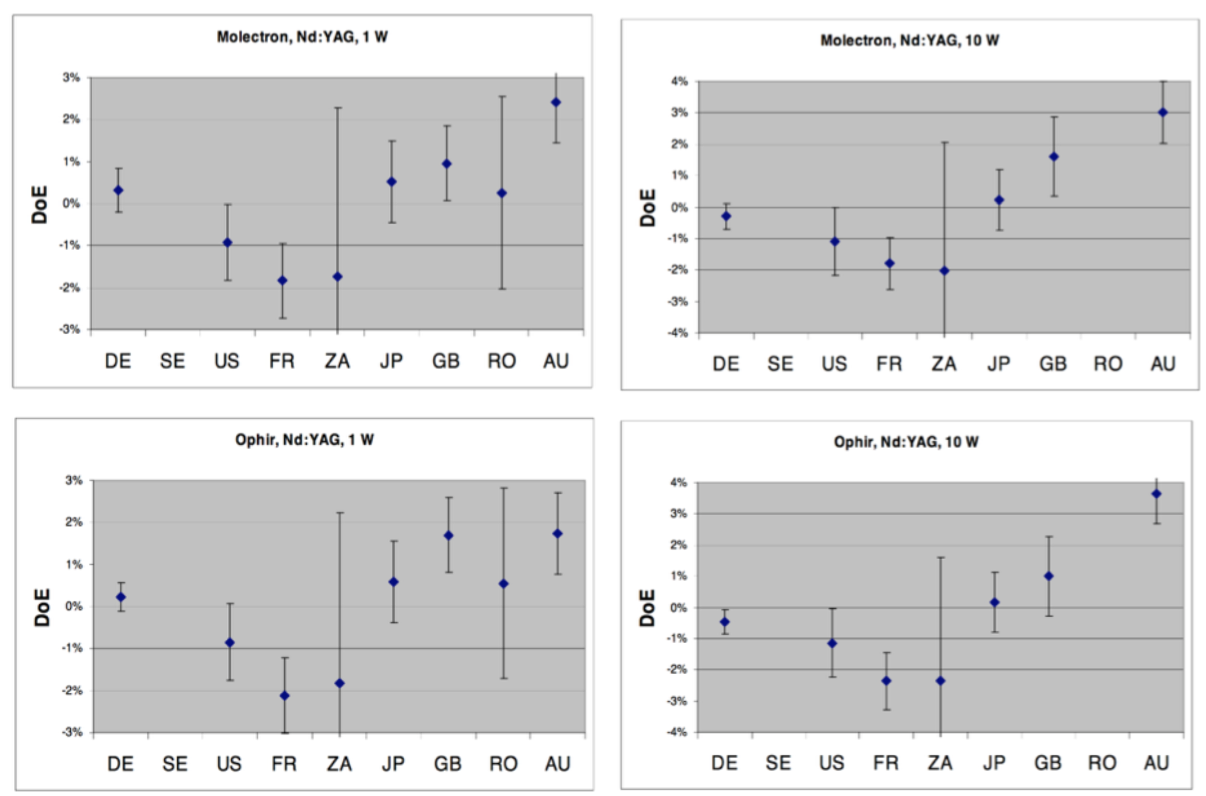
\includegraphics[width=14cm]{Figures/Power_standard.eps}
\caption{
Performance comparison of laser power standard system at 1064nm wavelength and 1W power in the national standard institutions in the world~\cite{EUROMET}.
} 
\label{fig:Power_standard} 
\end{center}
\end{figure}

\section{Crosscheck WS}
